\chapter{User Study}
\label{userStudy}

\section{Structure} We created a multi-phase user study to examine the correctness of our method of word frequency metric generation, which uses the UNISYN dictionary. 

First, we generated oronyms for the phrases ``a nice cold hour'' and ``fourth rye to''. Using the selection criteria outlined in section ~\ref{subsection:firstWaveUserStudy}, we narrowed down our recording options to \phaseOneANiceColdHourOronymsRecordedUnique out of the \aNiceColdHourOronymCount oronyms generated for ``a nice cold hour'', and \phaseOneFourthRyeToOronymsRecordedUnique out of the \forthRyeToOronymCount oronyms generated for ``fourth rye to''. 

In the first phase, we had \uniqueUsersPhaseOneUserStudy people record over \numResponsesPhaseOneUserStudy recordings of \phaseOneTotalOronymsRecordedUnique different phrases.  This phase served two purposes: one, to see if our phonemic transcriptions were valid, and two, to gather recordings for the second phase.  

In the second phase, we took \recordingsPhaseTwoUserStudy recordings of oronyms from phase one, and gathered \numTranscriptionsPerRecordingPhaseTwoUserStudy transcriptions for each recording, resulting in a total of \numResponsesPhaseTwoUserStudy transcriptions. These transcriptions were provided by \uniqueUsersPhaseTwoUserStudy unique users ( \uniqueUsersPhaseTwoUserStudyUSA from the United States).  We then compared the observed frequency of transcriptions of the recorded oronym phrases to the calculated frequency metric for oronyms of the original root phrase.

\section{User Sampling Population}
We drew our test subjects from a pool of Amazon Mechanical Turk workers (hired for \$ 0.02 to \$ 0.10 per task) and, for part of phase 1, volunteers from Reddit.com \cite{redditAssistance} \cite{redditRecordThis}. 

Amazon Mechanical Turk is an online crowdsourcing service where requesters can hire workers to complete Human Intelligence Tasks, or HITs.  The efficacy of using Mechanical Turk for user studies has been widely studied in academia, and specifically proven in the linguistic community \cite{sprouse_validation_2011}.

Due to the online nature of Mechanical Turk, we we able to gather an international pool of volunteers. As you can see in figure ~\ref{fig:responsesPerCountry}, the bulk of our responses came from the United States and India.


\section{Methodology}

\subsection{First Phase: Recitation}
\label{subsection:firstWaveUserStudy}
In this phase of the user study, we used a combination of \uniqueUsersPhaseOneUserStudy Mechanical Turk workers (hired for \$ 0.10 per task) to record \numResponsesPhaseOneUserStudy different phrases.  These phrases were oronyms of one of two phrases: phrase A, ``a nice cold hour'' or phrase B, ``fourth rye to''.  

Given that ``a nice cold hour'' has \aNiceColdHourOronymCount oronyms, and ``fourth rye to'' has \forthRyeToOronymCount, it was necessary to narrow down the number of oronyms recorded in phase one of our user study.  

To select which oronyms we would submit to Mechanical Turk for workers to record, we decided on the following selection criteria:
\begin{itemize}
\item We discarded oronyms that included words with frequency values of less than 30.  Asking a general audience to pronounce uncommon words would likely result in a high rate of unusable recordings. In addition, including uncommon words wouldn’t be testing our algorithm---it would be testing the vocabulary of the user study subjects, which is outside the scope of this project.
\item We discarded all oronym phrases that contained words that capitalize to proper nouns, if that capitalization leadto alternative pronunciations.  For example, ``nice'' maps to the phonetic sequence \texttt{n aI s}, but ``Nice'' maps to the phonetic sequence \texttt{n i s} (as in ``niece'') .  
\item We discarded oronym phrases that included implicit punctuation. For example, the phrase ``Anne I scold our'', has an implicit comma between Anne and I.  We did this to avoid halting or ``dramatic'' recording of phrases.
\item We discarded oronyms with any words whose pronunciation is position specific. For example, the word `` 'n' '' is pronounced \texttt{@ n} when found in ``Rock 'n' Roll’’, but when on its own, is pronounced \texttt{ E n}, which doesn't map back to the original root phrase ``an ice cold hour''. We also removed some phrases involving the word  `` o' ''.  When pronounced \texttt{@}, as it is in ``top o' the morning'', it maps back to the original root phrase, but when found outside of that phrase, as in a last name like O'Donnell, it is pronounced \texttt{ oU }, and doesn't map back.
\item We only chose oronyms for which all pronunciations of the child oronym phrases were also found in the pronunciations of the root oronym phrase. For example, a root phrase that begins with ``a'' would have an child oronym phrase that begins with ``et'', using French pronunciation which drops the trailing \texttt{t} sound. However, ``et'' can also be pronounced with the \texttt{t}, using an American accent, as in the phrase ``et al''. Since our root phrase doesn’t include that \texttt{t} sound, any child oronym phrases that begin with ``et'' have at least one pronunciation that does not match the root phrase's pronunciation.  So, we discard all child oronyms that begin with ``et''.
\end{itemize}

At the end of this process, we were left with \phaseOneANiceColdHourOronymsRecordedUnique out of the \aNiceColdHourOronymCount oronyms generated for ``a nice cold hour'', and \phaseOneFourthRyeToOronymsRecordedUnique out of the \forthRyeToOronymCount oronyms generated for ``fourth rye to''. 


To keep track of the chosen phrases, we assigned each phrase an phraseID, built off of the phrase letter, phrase length, and phrase text. We gave Mechanical Turk workers three minutes to record each phrase and email it to us with the phrase identifier in the subject of the email. The number of recordings per phrase, along with their identifiers, can be seen in table ~\ref{table:phrasesRecorded}.

We then interpreted the phonetics of each of the recordings in SAMPA by ear.  In a stunning example of a use case for our project, we discovered that we had unintentionally included some phrases for recording which were not deterministically phonetically parsible, meaning that our oronyms had multiple pronunciations, not all of which mapped back to the original phrase.  While we had caught and removed the phrases that began with ``et'', our algorithm mapped the orthographic word ``a'' to the phoneme \texttt{A} (as in ``a capella'' or ``f\emph{a}ther''. That \texttt{A} phoneme can be combined with the subsequent \texttt{n} phoneme from the word ``nice'' to create the SAMPA sequence \texttt{A n}, which corresponds with the orthographic word ``on''.  Since that doesn't map back to our original root phrase, we were forced to discard all transcriptions that ended up with that pronunciation. That being said, the remaining pronuciations fit with our model, and we found no unexpected phonetic anomalies when comparing our recordings to the expected SAMPA pronunications of each phrase.



\subsection{Recording Sample Pool}
\label{subsection:recordingSamplePool}
We had originally intended to use all the phase one recordings in phase two, but had to discard all but \recordingsPhaseTwoUserStudy of the recordings for various reasons, the most common being that the recording was too loud and we wanted to spare our user's ears. Occasionally, the person recording left excessive amounts of space between words that overly-segmented the phrase, interrupting the natural flow of the phonetic sequence and rendering it unusable for our purposes.  The recordings for the ``fourth rye to" oronyms were all unusable for phase two, because our users tended to insert exclamation points any time they said ``ooh" or ``too", overloading their microphones or over-segmenting the phrase.

All \recordingsPhaseTwoUserStudy recordings we used were oronyms for the phrase ``a nice cold hour", and were recorded by one man from the midwest, whose accent which made him the best approximation we could get for a General American accent. All other recordings gathered in phase one did not have appropriate accents, and were summarily discarded from further data collection.

\subsection{Second Wave: Transcription}
\label{subsection:secondWaveUserStudy}

We hired \uniqueUsersPhaseTwoUserStudy unique Mechanical Turk workers to transcribe our oronym recordings for \$ 0.02 to \$ 0.03 per transcription.  Each of the \recordingsPhaseTwoUserStudy recordings was transcribed \numTranscriptionsPerRecordingPhaseTwoUserStudy times, resulting in a total of \numResponsesPhaseTwoUserStudy transcriptions. These transcriptions were provided by \uniqueUsersPhaseTwoUserStudy unique users ( \uniqueUsersPhaseTwoUserStudyUSA from the United States). In addition to transcribing the recording, in each task the worker was asked what country they were from. We did this to help differentiate native American English speakers from non-native speakers.

\begin{figure}
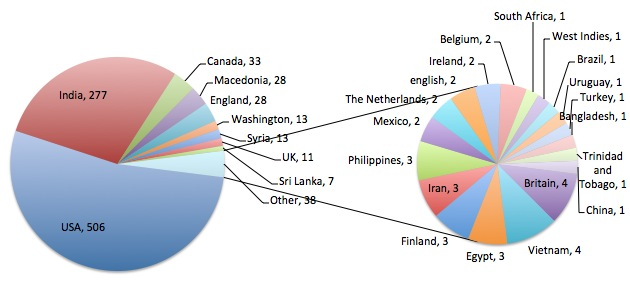
\includegraphics[width=150mm]{responsesPerCountry.jpg}
\captionfonts
\caption[Responses Per Country]{ Our user study primarily polled people from the United States and India, as can be seen by the number of responses originating from each country. }
\label{fig:responsesPerCountry}
\end{figure}



